W tym rozdziale przedstawiono projekt systemu, który ma zostać zaimplementowany na potrzeby tej pracy. Projektowany system powinien umożliwiać uruchomienie aplikacji na dowolnie dużym klastrze obliczeniowym składającym się z maszyn o różnej specyfikacji. Na komputerze, na którym aplikacja jest uruchamiana (a więc tym wykorzystywanym przez użytkownika) powinno uruchomić się okno dające podgląd na generowaną animację. Aplikacja powinna dawać możliwość załadowania pliku opisującego scenę, która następnie będzie rozesłana do wszystkich węzłach klastra. Opis działania klastra i planowanych klas programu (powiązania między nimi i rola w systemie) został umieszczony poniżej. 

\section{Projekt klastra}

\begin{figure}[h!]
\centering
  \caption{Schemat systemu}
  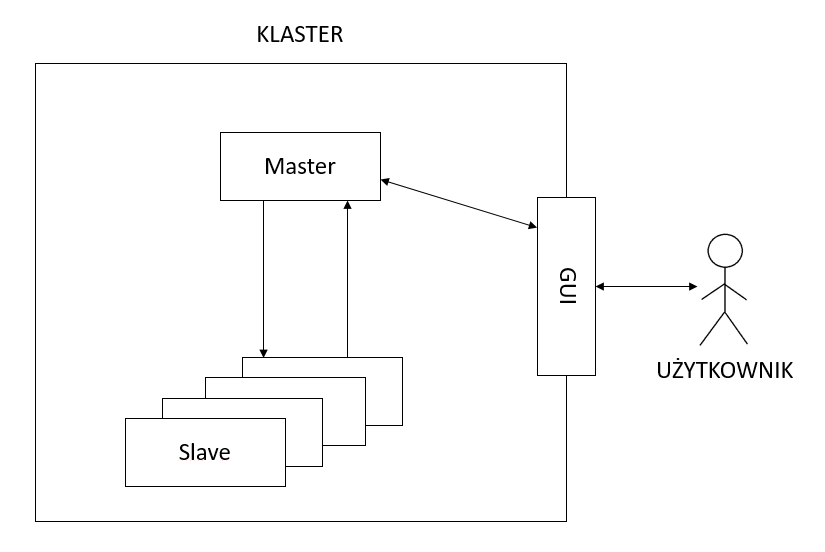
\includegraphics[width=10cm]{cluster.png}
\end{figure}

Na powyższym schemacie przedstawiono konceptualny schemat działania systemu. W założeniach, użytkownik ma komunikować się z klastrem poprzez graficzny interfejs użytkownika (zbudowany z wykorzystaniem biblioteki Qt), który udostępni mu podgląd dynamiczne budowanej animacji i wszelkich statystyk z nią związanych. Program master'a (a więc głównego węzła klastra) ma wykonywać się na tej samej maszynie, która udostępnia interfejs - główny proces zostanie podzielony na dwa wątki: jeden zajmujący się obsługą klastra (wątek master'a) i drugi związany z użytkownikiem (wątek GUI). Węzeł zarządzający komunikuje się z każdym z węzłów wykonawczych, zlecając im zadania i zbierając od nich wyniki. W chwili, w której zostanie wygenerowana cała klatka, master informuje wątek GUI, o tym że wygenerowany obraz jest gotowy do wyświetlenia. W poniższych punktach zostanie zaprezentowany proponowany algorytm zachowania węzłów.  
	
\subsection{Master}

Pierwszym i najważniejszym zadaniem węzła zarządzającego jest wczytanie pliku zawierającego definicję generowanego obrazu. Na podstawie pliku wejściowego ma on stworzyć scenę, kamerę, obiekty i światła. Następnie musi on rozesłać informacje na temat obiektów do wszystkich węzłów wykonawczych, tak aby każdy z nich posiadał tę samą definicję obrazu (broadcast). Gdy już każdy z węzłów zasygnalizuje gotowość, węzeł zarządzający rozsyła zadania policzenia danego wycinka obrazu do węzłów wykonawczych. Poniżej przedstawiono przykładowy pseudokod działania master'a. Warto zwrócić uwagę, że zadania umieszczane są na kolejce oczekującej - takie rozwiązanie powinno dawać lepsze rezultaty niż rozesłanie wszystkim węzłom wszystkich zadań od razu, ponieważ różne fragmenty obrazu mogą być generowane z różną prędkością. Mogłoby więc dochodzić do sytuacji, w której część węzłów zrealizowało już swoje zadania (a więc ich moc obliczeniowa nie jest wykorzystywana), a część (która dostała bardziej wymagające obliczenia) ciągle liczy.

\begin{algorithm}
\begin{algorithmic}
\State readFile()
\State sendScene()
\State sendCamera()
\\
\While{true}
\\
\State queue = splitImageToChunks()
\State //pending - liczba zleconych, niewykonanych zadań
\State pending = sendChunkToEveryNode()
\\
\While {pending $>$ 0}
\State msg = recvMessage()
\If {msg == EXIT} exit()
\ElsIf {msg = PIXELS}
	recvPixels()
	\If {queue is not empty}
		sendChunkToSlave()
	\Else
		pending--
	\EndIf
\EndIf
\EndWhile
\State informGUI()
\State updateCameraPos()
\EndWhile
\end{algorithmic}
\end{algorithm}


\subsection{Slave}

Nawiązując do poprzedniego punktu, pierwszą czynnością, którą powinien wykonać każdy ze slave'ów jest odebranie definicji obiektów wykorzystywanych przy generowaniu sceny. Następnie w pętli, może on czekać na zadanie, realizować je (z wykorzystaniem klasy RayTracer) i odsyłać z powrotem do węzła zarządzającego.

\begin{algorithm}
\begin{algorithmic}
\State recvScene()
\State recvCamera()
\\
\While{true}
\State msg = recvMessage()
\If {msg == EXIT} exit()
\ElsIf {msg == CHUNK}
	recvChunk()
	pixels = recursiveRayTracer()
	sendPixels()
\ElsIf {msg == CAMERA}
	recvCamera() //aktualizacja pozycji kamery
\EndIf
\EndWhile
\end{algorithmic}
\end{algorithm}


\section{Projekt programu}

	\subsection{Diagram klas}
	\begin{figure}[H]
    \centering
              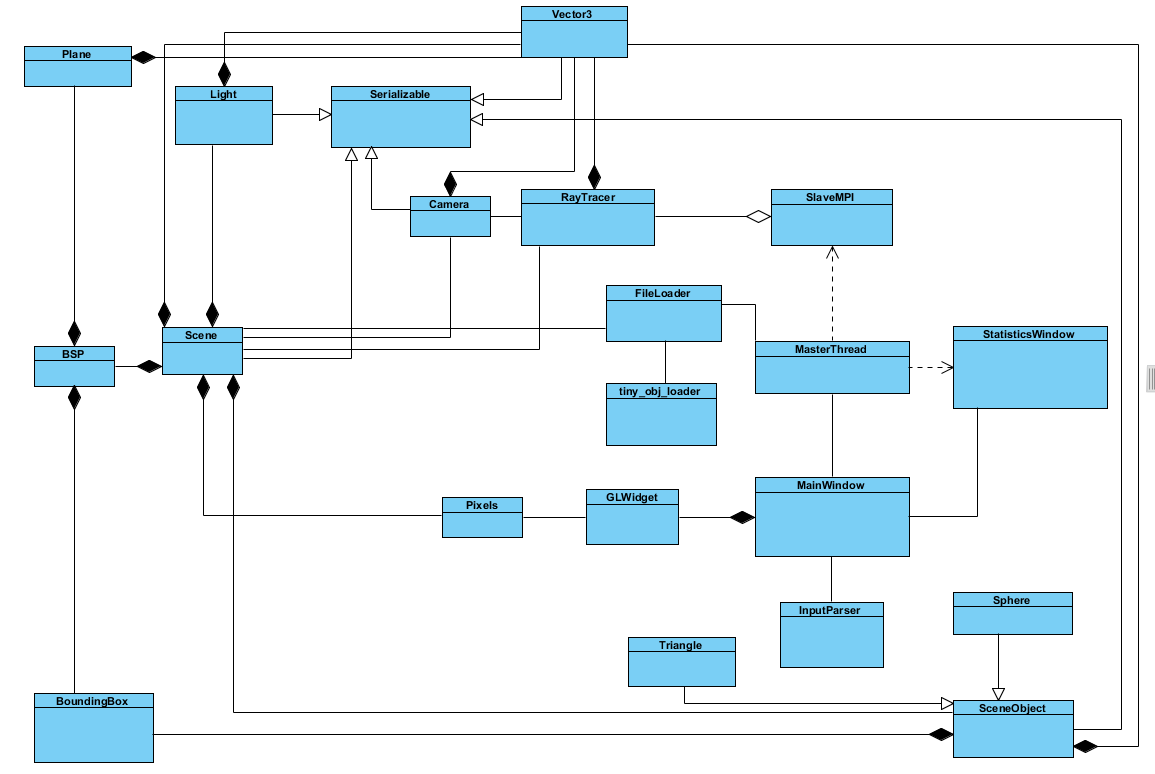
\includegraphics[angle=90,width=\textwidth,
                    height=0.8\textheight,
                   ]{classDiagram.PNG}
    \caption{Diagram klas}
    \label{fig:classDiagram}
	\end{figure}
	
	Powyżej przedstawiono uproszczony diagram klas. Opis poszczególnych z nich (wraz ze spisem atrybutów i metod) znajduje się w kolejnym podrozdziale.
	
\subsection{Opis klas}

\subsubsection{BoundingBox}


\footnotesize
\footnotesize
\begin{longtable}{|p{14cm}|}
	\caption{BoundingBox} \label{tab:BoundingBox} \\ \hline
	\multicolumn{1}{|c|}{BoundingBox} \\ \hline
    +minX : float \\
    +maxX : float \\
    +minY : float \\
    +maxY : float \\
    +minZ : float \\
    +maxZ : float \\ \hline
    +intersect(start: Vector3, dir: Vector3 \\ \hline
\end{longtable}
\normalsize

Klasa BoundingBox reprezentuje prostopadłościany, które w założeniu mają otaczać inne obiekty (bryła otaczająca). Ma ona umożliwić przyspieszenie badania przecięcia promieni z elementami sceny (stąd metoda intersect). W programie będzie wykorzystywana przez drzewo BSP (otoczenie całej sceny) i SceneObject. 


\subsubsection{BSP}

\footnotesize
\footnotesize
\begin{longtable}{|p{14cm}|}
	\caption{BSP} \label{tab:BSP} \\ \hline
	\multicolumn{1}{|c|}{BSP} \\ \hline

    +tree : node* \\
    -polygons : SceneObject* \\
    -box : BoundingBox \\ \hline
    +build(root : node*, polygons : SceneObject*, depth : int) \\ 
	-getBestPlane(polygons : list$<$SceneObject*$>$) : Plane \\
	+getClosest(cross : Vector3, start : Vector3, dir : Vector3) : SceneObject* \\
	+isInShadow(cross : Vector3, dir : Vector3, light : Vector3) : bool \\
	-getBoundingBox(polygons : list$<$SceneObject*$>$) : BoundingBox \\
	-intersect(root : node*, cross : Vector3, start : Vector3, dir : Vector3) : SceneObject* \\
	-deleteTree(root : node*) : void \\
    \hline
\end{longtable}
\normalsize

\footnotesize
\begin{longtable}{|p{14cm}|}
    \caption{Node} \label{tab:Node} \\ \hline
    \multicolumn{1}{|c|}{Node} \\ \hline
    partitionPlane : Plane \\
    polygons : list$<$SceneObject*$>$ \\
    front : node*  \\
    back : node*  \\ \hline
\end{longtable}
\normalsize

Klasa BSP implementuje drzewo opisane w rozdziale (!RODZIAŁ!). Poza metodami związanymi z budową drzewa, zawiera ona metody analogiczne do Klasy Scene (z tą różnicą, że metody Scene wykorzystują przegląd zupełny obiektów) umożliwiające przeglądanie sceny w poszukiwaniu przeciętych obiektów i badania, czy dany punkt znajduje się w cieniu. Drzewo BSP jest składową klasy Scene, która wywołuje jego metody (jeżeli jest ustawiona flaga mówiąca o wykrzystaniu drzewa).

Podstawowym elementem drzewa jest struktura Node, która zawiera pola takie jak płaszczyzna podziału, wskaźniki na kolejne wierzchołki drzewa (reprezentujące przestrzeń przed i za płaszczyzną) i listę obiektów należących do danego wierzchołka. Obiekt może należeć do wierzchołka np. w sytuacji gdy wierzchołek jest liściem lub obiekt leży na płaszczyźnie podziału. Klasa BSP zostanie dokładniej opisana w rozdziale 6.


\subsubsection{GLwidget}

\footnotesize
\begin{longtable}{|p{14cm}|}
    \caption{GLwidget} \label{tab:GLwidget} \\ \hline
    \multicolumn{1}{|c|}{GLwidget} \\ \hline
    scene : Scene*  \\ \hline
    initializeGL() : void \\ 
    resizeGL(int w, int h) : void \\
    paintGL() : void \\ \hline
\end{longtable}
\normalsize

Widgety są składowymi elementami graficznego interfejsu użytkownika i nie wszystkie z nich muszą być reprezentowane poprzez obiekty. Klasa GLwidget odpowiada za prezentowanie kolejnych klatek użytkownikowi. W przypadku kiedy główne okno aplikacji (MainWindow, ,,rodzic'' GLwidget) otrzyma informacje o wygenerowaniu kolejnej klatki od MasterThread wywołuje odpowiednią metodę GLwidget - GLwidget odwołuje się do Klasy Scene od której otrzymuje tablicę pikseli (Pixels) do wyświetlenia. 

\subsubsection{FileLoader}

\footnotesize
\begin{longtable}{|p{14cm}|}
    \caption{FileLoader} \label{tab:FileLoader} \\ \hline
    \multicolumn{1}{|c|}{FileLoader} \\ \hline
    -readCameraSettings(line : char const*) : bool \\
    -readSceneSettings(line : char const*) : bool \\
    -readSphere(line : char const*) : bool \\
    -readLight(line : char const*) : bool \\
    -readTriangle(line : char const*) : bool \\
    -readObj(line : char const*) : bool \\
	+ReadFile(fname : char const*) : bool \\ \hline
\end{longtable}
\normalsize

FileLoader jest klasą odpowiedzialną za wczytanie definicji sceny z pliku (stąd powiązania z klasami Scene i Camera). Jest ona wykorzystywana przez klasę MasterThread. Klasa korzysta z biblioteki tinyobjloader dzięki której możliwe jest wczytywanie modeli zapisanych w formacie ,,obj''. Bibliotekę można znaleźć pod adresem https://github.com/syoyo/tinyobjloader. Jest ona udostępniona na licencji MIT.

\subsubsection{InputParser}

\footnotesize
\begin{longtable}{|p{14cm}|}
    \caption{InputParser} \label{tab:InputParser} \\ \hline
    \multicolumn{1}{|c|}{InputParser} \\ \hline
    tokens : vector$<$string$>$  \\ \hline
    +getCmdOption(option : string const) : string const) \\
    +cmdOptionExists(option : string const) : bool \\ \hline
\end{longtable}
\normalsize

Klasa InputParser jest prostą klasą pozwalająca na obróbkę danych wejściowych (dokładniej opisane w rozdziale !WSTAW RODZIAŁ!). Klasa MainWindow, która w założeniach ma tworzyć wątek MasterThread, wykorzystuje ją do przekazania mu parametrów.

\subsubsection{Light}

\footnotesize
\begin{longtable}{|p{14cm}|}
    \caption{Light} \label{tab:Light} \\ \hline
    \multicolumn{1}{|c|}{Light} \\ \hline
    +pos : Vector3* \\ 
    +amb : Vector3* \\
    +dif : Vector3* \\
    +spec : Vector3* \\
    \hline
	+serialize(bytes : vector$<$char$>$*) : void \\ 
	+deserialize(bytes : vector$<$char$>$ const) : void \\
	+getType() : char \\
	\hline
\end{longtable}
\normalsize

Klasa Light określa obiekty światła. Więcej o świetle i jego znaczeniu na scenie można przeczytać w rozdziale !ROZDZIAŁ!.

\subsubsection{MainWindow}

\footnotesize
\begin{longtable}{|p{14cm}|}
    \caption{MainWindow} \label{tab:MainWindow} \\ \hline
    \multicolumn{1}{|c|}{MainWindow} \\ \hline
    ui : MainWindow* \\
    statisticWindow : StatisticsWindow* \\
    masterThread : MasterThread* \ \
    statusLabel : QLabel* \\ \hline
    createMaster() \\
    ShowStats() \\
    setSpeed(double time) \\
    on\_actionStatistics\_triggered() \\
    onQuit(); \\ \hline
\end{longtable}
\normalsize

Klasa MainWindow reprezentuje główne okno aplikacji. Ze względów projektowych jest ona odpowiedzialna za tworzenie obiektu MasterThread (ma to związek z mechanizmem przypisania sygnałów do slotów - mechanizm komunikacji międzywątkowej w Qt) jak i potrzebie komunikacji między jedną i drugą klasą. Klasa MainWindow (wraz z GLwidget i StatisticWidnow) reprezentuje warstwę prezentacji tworzonej aplikacji.

\subsubsection{MasterThread}

\footnotesize
\begin{longtable}{|p{14cm}|}
    \caption{MasterThread} \label{tab:MasterThread} \\ \hline
    \multicolumn{1}{|c|}{MasterThread} \\ \hline
    isAlive : bool \\
    camera : Camera* \\
    scene : Scene* \\
    processSpeed : double** \\
    worldSize : int \\
    status : MPI\_Status \\
    names : vector$<$string$>$ \\
    pending : int \\
    numChunks : int \\
    queue : queue$<$Chunk$>$ \\
    test : int \\
    \hline
	run() \\
	splitToChunks(int num) \\
	clearQueue(queue$<$Chunk$>$ q) \\
    sendCameraBcast() \\
    sendCameraPointToPoint() \\
    sendScene() \\
    sendDepth(int depth) \\
    sendNextChunk(int dest) \\
    sendExitSignal() \\
    recvPixels(MPI\_Status stat) : int \\
    recvMessage() : int \\
    finishPending() \\
    updateProcessSpeed() \\
    waitUntillRdy() \\
    printResult(double spf, double bsp) \\
    getNames() \\
    emitNames() \\
	\hline
\end{longtable}
\normalsize

Główna klasa aplikacji, której obiekt tworzony jest w tym samym procesie co MainWindow, jednak działający w osobnym wątku. Takie rozwiązanie pozwala zachować responsywność aplikacji. Wątek okna głównego jest odpowiedzialny za przetwarzanie zdarzeń wygenerowanych przez użytkownika czy program, a wątek MasterThread, niezależnie od niego, zajmuje się w tym czasie generowaniem kolejnej klatki animacji. Rozdzielamy w ten sposób warstwę prezentacji od warstwy biznesowej tworząc tym samym aplikację przyjaźniejszą użytkownikowi.

Głównym zadaniem MasterThread jest zarządzanie węzłami wykonawczymi (sami stanowi serce węzła nadzorującego). Posiada on szereg metod umożliwiających komunikację z innymi procesami tworzącymi aplikację. Ma on dostęp do lokalnych kopii obiektów Scene i Camera, ponieważ musi je rozesłać po klastrze i mieć możliwość modyfikacji ich parametrów (przesunięcie kamery co klatkę, aktualizacja obiektu Pixels). Więcej o zadaniach i sposobie działania MasterThread można przeczytać (!rodział z wyżej!, !rodział z implementacji!).

\footnotesize
\begin{longtable}{|p{14cm}|}
    \caption{Chunk} \label{tab:Chunk} \\ \hline
    \multicolumn{1}{|c|}{Chunk} \\ \hline
    startx : int \\
    stopx : int \\
    starty : int \\
    stopy : int \\
    \hline
\end{longtable}
\normalsize

Chunk jest prostą strukturą wykorzystywaną w komunikacji Master/Slave (MasterThread, SlaveMPI). Zawiera on w sobie informacje o tym jaki wycinek obrazu powinien być wyznaczany przez dany węzeł wykonawczy.


\subsubsection{Pixels}

\footnotesize
\begin{longtable}{|p{14cm}|}
    \caption{Pixels} \label{tab:Pixels} \\ \hline
    \multicolumn{1}{|c|}{Pixels} \\ \hline
    +data : unsigned char* \\
    +x : int \\
    +y : int \\ 
    +startx : int \\
    +starty : int \\
    \hline
	+serialize(bytes : vector$<$char$>$*) : void \\
	+deserialize(bytes : vector$<$char$>$ const) : void \\
	+getType() : char \\
	+setStartXY(x : int, y : int) : void \\
	+setPixel(posX : int, posY : int, vec : Vector3) : void \\
	\hline
\end{longtable}
\normalsize

Klasa Pixels przechowuje tablice pikseli w formie ciągu bajtów unsigned char* (taka reprezentacja jest wykorzystywana przez funkcje rysujące, które zapewniają przyspieszenie sprzętowe). Pozwala ona stworzyć wygodny interfejs czytania i pisania do tablicy. 

\subsubsection{Plane}

\footnotesize
\begin{longtable}{|p{14cm}|}
    \caption{Plane} \label{tab:Plane} \\ \hline
    \multicolumn{1}{|c|}{Plane} \\ \hline
    +a : float \\ 
    +b : float \\
    +c : float \\
    +d : float \\
    \hline
	+classifyObject(obj : SceneObject*) : int \\
	+classifyPoint(point : Vector3*) : int \\
	+getDistToPoint(point : Vector3*) : float \\
	+rayIntersectPlane(start : Vector3, dir : Vector3) : bool \\
	+getNormal() : Vector3 \\
	+isValid() : bool \\
	\hline
\end{longtable}
\normalsize

Klasa reprezentuje obiekty płaszczyzn, wykorzystywane przy podziale podprzestrzeni przez drzewo BSP. Zawiera metody pozwalające określić po której stronie płaszczyzny znajduje się dany obiekt.

\subsubsection{RayTracer}

\footnotesize
\begin{longtable}{|p{14cm}|}
    \caption{RayTracer} \label{tab:RayTracer} \\ \hline
    \multicolumn{1}{|c|}{RayTracer} \\ \hline
    +camera : Camera* \\
    +scene : Scene* \\ \hline
	+basicRayTracer() : void \\
	+recursiveRayTracer(depth : int) : void \\
	+getColorRecursive(start : Vector3, dir : Vector3, depth : int) : Vector3 \\
	\hline
\end{longtable}
\normalsize

Klasa RayTracer zawiera w sobie zestaw metod, które pozwalają na realizację algorytmu śledzenia promieni. W tym celu odwołuje się ona do pól klasy Scene i Camera. Każdy obiekt SlaveMPI (zawierający w sobie algorytm działający na węzłach wykonawczych) tworzy własny obiekt RayTracer'a. Klasa ta zostanie dokładniej opisana w rozdziale 6.

\subsubsection{Scene}

\footnotesize
\begin{longtable}{|p{14cm}|}
    \caption{Scene} \label{tab:Scene} \\ \hline
    \multicolumn{1}{|c|}{Scene} \\ \hline
    +numOfLights : int \\
    +numOfObjects : int \\
    +useShadows : bool \\
    +useBSP : bool \\
    +instance : Scene* \\
    +lights : Light** \\
    +sceneObjects : SceneObject** \\
    +pixels : Pixels* \\
    +backgroundColor : Vector3* \\
    +globalAmbient : Vector3* \\
    +bsp : BSP* \\
    \hline
	+getInstance() : Scene * \\
	+buildBSP(depth : int) : void \\
	+addObject(sceneObject : SceneObject*) : void \\
	+addLight(light : Light*) : void \\
	+setUpPixels(x : int, y : int) : void \\
	+getClosest(cross : Vector3, start : Vector3, dir : Vector3) : SceneObject * \\
	+isInShadow(cross : Vector3, dir : Vector3, lightPos : Vector3) : bool \\
	+setPixelColor(x : int, y : int, color : Vector3) : void \\
	+serialize(bytes : vector$<$char$>$*) : void \\
	+deserialize(bytes : vector$<$char$>$ const) : void \\
	+getType() : char \\
	\hline
\end{longtable}
\normalsize

Obiekt zawierający definicję całej sceny. Jest on napisany według wzorca Singleton (może istnieć tylko jeden obiekt takiej klasy). Wywołując statyczną metodę getInstance() otrzymamy na niego wskaźnik. Obiekt Scene jest jednym z częściej wykorzystywanych obiektów, gdyż jest centralnym elementem aplikacji - zawiera pola istotne dla wielu klas. W związku z tym udostępnia on interfejs pozwalający na pobieranie interesujących daną klasę danych (np. metoda isInShadow, która bada czy dany punk znajduje się w cieniu. Klasa, zgodnie z flagą useBSP, dokonuje przeglądu zupełnego, lub wykorzystuje drzewo).

\subsubsection{SceneObject}

\footnotesize
\begin{longtable}{|p{14cm}|}
    \caption{SceneObject} \label{tab:SceneObject} \\ \hline
    \multicolumn{1}{|c|}{SceneObject} \\ \hline
    \#specShin : float \\
    \#transparency : float \\
    \#mirror : float \\
    \#local : float \\
    \#density : float \\
    \#amb : Vector3* \\
    \#dif : Vector3* \\
    \#spec : Vector3* \\
    \hline
	+getLocalColor(normal : Vector3, cross : Vector3, observation : Vector3) : Vector3 \\
	+trace(cross : Vector3, start : Vector3, dir : Vector3, dist : float) : bool \\
	+getNormalVector(cross : Vector3) : Vector3 \\
	+getBoundingBox() : BoundingBox \\
	\hline
\end{longtable}
\normalsize

SceneObject jest wirtualną klasą po której powinny dziedziczyć wszystkie obiekty sceny. Pozwala on na wykorzystywanie wielopostaciowości (widoczne np. w klasie Scene), wymuszając na klasach potomnych implementacje metod pozwalających określić przecięcie z promieniem (trace()), oblicznie wektora normalnego w punkcie (getNormalVector()), czy pobranie koloru w punkcie (getLocalColor())

\subsubsection{Serializable}

\footnotesize
\begin{longtable}{|p{14cm}|}
    \caption{Serializable} \label{tab:Serializable} \\ \hline
    \multicolumn{1}{|c|}{Serializable} \\ \hline
    +serializedSize : int \\ \hline
	+serialize(bytes : vector$<$char$>$*) : void \\ 
	+deserialize(bytes : vector$<$char$>$ const) : void \\
	+getType() : char \\
	\hline
\end{longtable}
\normalsize

Klasa Serializable jest właściwie Interfejsem - dziedziczą po niej wszystkie klasy, które muszą mieć możliwość serializacji (zamiana obiektu na ciąg bajtów) w związku z potrzebą wysłania ich do innych węzłów klastra. Bardziej szczegółowe informacje o serialializacji można znaleźć w rodziale 6.

\subsubsection{SlaveMPI}

\footnotesize
\begin{longtable}{|p{14cm}|}
    \caption{SlaveMPI} \label{tab:SlaveMPI} \\ \hline
    \multicolumn{1}{|c|}{SlaveMPI} \\ \hline
    +x : int \\ 
	+y : int \\
	+depth : int \\
	+status : MPI\_Status \\
	+pixels : Vector3*** \\
	+camera : Camera* \\
	+scene : Scene* \\ \hline
	+exec() : int \\
	+recvCameraBcast() : void \\
	+recvCameraPointToPoint() : void \\
	+recvScene() : void \\
	+recvDepth() : void \\
	+recvChunk() : void \\
	+recvMessage() : int \\
	+sendPixels() : void \\
	+sendName() : void \\
	+sendRdy() : void \\
	\hline
\end{longtable}
\normalsize

SlaveMPI jest klasą analogiczną do klasy MasterThraed, jednak jej obiekt jest tworzony na każdym węźle wykonawczym. Zawiera ona w sobie metody implementujące mechanizmy komunikacji z resztą węzłów i takie pozwalające na wykonywanie zadań zleconych przez mastera  Metoda exec() implementuje algorytm opisany w rozdziale (!wstaw rozdział!) - główną pętlę programu węzłów wykonawczych. Więcej o implementacji można znaleźć w rozdziale 6.

\subsubsection{StatisticsWindow}

\footnotesize
\begin{longtable}{|p{14cm}|}
    \caption{StatisticsWindow} \label{tab:StatisticsWindow} \\ \hline
    \multicolumn{1}{|c|}{StatisticsWindow} \\ \hline
    Ui::StatisticsWindow *ui; \\
    int worldSize; \\
    \hline
	resizeEvent(QResizeEvent *event) : void \\
    setTime(double time) : void  \\
    setChunks(int i) : void \\
    setXY(int x, int y) : void \\
    setObj(int i) : void \\
    setLights(int i) : void  \\
    setProccessName(int num, QString str) : void \\
    setProccessSpeed(double **speed) : void \\
    setUpList() : void \\
    \hline
\end{longtable}
\normalsize

StatisticWindow jest oknem, które (jak sama nazwa wskazuje) ma prezentować statystki dot. programu - czas generowania jednej klatki, średni czas pracy danego węzła, liczbę obiektów na scenie itd.

\subsubsection{Sphere}

\footnotesize
\begin{longtable}{|p{14cm}|}
    \caption{Sphere} \label{tab:Sphere} \\ \hline
    \multicolumn{1}{|c|}{Sphere} \\ \hline
    +radius : float \\
    +pos : Vector3* \\
    \hline
\end{longtable}
\normalsize

Klasa Sphere jest klasą reprezentującą sferę. Dziedziczy ona po SceneObject, a więc implementuje metody specyficzne dla tego typu obiektu (np. badanie przecięcia z obiektem).

\subsubsection{Triangle}

\footnotesize
\begin{longtable}{|p{14cm}|}
    \caption{Triangle} \label{tab:Triangle} \\ \hline
    \multicolumn{1}{|c|}{Triangle} \\ \hline
    +pointA : Vector3* \\
    +pointB : Vector3* \\
    +pointC : Vector3* \\
    +normalA : Vector3* \\
    +normalB : Vector3* \\
    +normalC : Vector3* \\
    \hline
	+split(plane : Plane, front : list$<$Triangle*$>$, back : list$<$Triangle*$>$) : void \\ 
	+getPointbyNum(a : int) : Vector3 * \\
	+getPlanes() : list$<$Plane$>$ \\
	+getPerpendicularPlane(i : int) : Plane \\
	+getPlane() : Plane \\
	+Area(a : Vector3, b : Vector3) : float \\
	+getBoundingBox() : BoundingBox \\
	\hline
\end{longtable}
\normalsize

Triangle jest klasą reprezentującą obiekty trójkąta. Triangle podobnie jak Sphere dziedziczy po SceneObject i implementuje metody specyficzne dla tego typu obiektu.

\subsubsection{Vector3}

\footnotesize
\begin{longtable}{|p{14cm}|}
    \caption{Vector3} \label{tab:Vector3} \\ \hline
    \multicolumn{1}{|c|}{Vector3} \\ \hline
    +x : type \\
    +y : type \\
    +z : type \\
     \hline
	+normalize() : Vector3 \\ 
	+scalarProduct(v : Vector3) : float \\
	+vectorProduct(v : Vector3) : Vector3 \\
	+rotateX(alpha : float) : void \\
	+rotateY(alpha : float) : void \\
	+rotateZ(alpha : float) : void \\
	+distanceFrom(v : Vector3) : float \\
	+powDistanceFrom(v : Vector3) : float \\
	+reflect(n : Vector3) : Vector3 \\
	+refract(normalVector : Vector3, a : float, b : float) : Vector3 \\
	+isZeroVector() : bool \\
	+length() : float \\
	\hline
\end{longtable}
\normalsize

Klasa Vector3 jest klasą pozwalającą definiować obiekty takie jak punkt, czy wektor w przestrzeni 3D. Zapewnia ona szereg metod implemetnujących różne operacje matematyczne na tego typu obiektach. Poza wszystkimi metodami wymienionymi wyżej zostanie również przeciążonych wiele operatorów arytmetycznych.
